\documentclass[paper=a4,fontsize=11pt]{includes}

% Set to true for english or false for spanish
\setboolean{en}{false}

\begin{document}

%%% My info
%%% ------------------------------------------------------------

\begin{minipage}{.2\linewidth}
   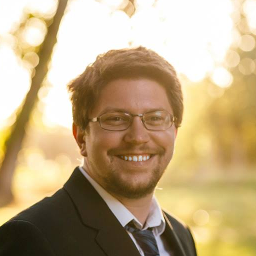
\includegraphics[width=1\textwidth]{img/photo}
\end{minipage}
\begin{minipage}{0.7\linewidth}
   \MyName{Christopher Barry Cromer}
   \sepspace
   \noindent

   \hfill +569 90864256

   \hfill chris@cromer.cl

   \hfill www.cromer.cl
\end{minipage}

%%% Work experience
%%% ------------------------------------------------------------

\NewPart{Work Experience}{Experiencia Laboral}
\noindent

\WorkEntry
{University of the Bío Bío}{Universidad del Bío Bío}
{Networking and Systems Engineer}{Ingeniero de Redes y Sistemas}
{Sep 2017 - Current}{Sep 2017 - Actual}
{I designed the local network used en the computer laboratory of the construction department of the\
    university. I maintained the servers in the laboratory. I provided technical support for the
    laboratory.}
{Diseñé la red interna del laboratorio de computación en el departamento de construcción de la\
    universidad. Mantuvé los servidores del laboratorio. Proporcioné soporte técnico para el laboratorio.}
{img/ubb}

\sepspace

\WorkEntry
{Oval}{Oval}
{Freelancer}{Freelancer}
{Jul 2019 - Sep 2019}{Jul 2019 - Sep 2019}
{I implemented some new areas in their internal platform used for managing contractors. I optimized various parts of the platform to run more\
    efficiently and load quicker.}
{Implementé algunas áreas nuevas en su plataforma interna utilizadas para la gestión de contratistas. Optimicé varias partes de la plataforma\
    para que funcione de manera más eficiente y cargue más rápido.}
{img/oval}

\sepspace

\WorkEntry
	{Tronwell}{Tronwell}
	{IT Manager}{Gerente de Informática}
	{Dec 2012 - Nov 2014}{Dic 2012 - Nov 2014}
	{I was responsible for maintaining the computer systems and server at the Concepción office. I designed\
		various interal software and mobile applications for them. I also provided technical support for the\
		offices in Concepción, Chillan, and Los Ángeles.}
	{En este trabajo fui responsable de mantenimiento de los sistemas informáticos y sus servidores de la\
		sede en Concepción. Desarrollé varios sistemas internos y aplicaciones para móviles. También\
		proporcioné soporte técnico para Concepción, Chillan y Los Ángeles.}
	{img/tronwell}

\sepspace

\WorkEntry
	{Best Buy}{Best Buy}
	{Computer Supervisor}{Supervisor}
	{Sep 2005 - Nov 2010}{Sep 2005 - Nov 2010}
	{I was the supervisor of the computer deparment at the Best Buy in Pensacola. In this role I had to\
		train develop, and supervise my employees}
	{Fui supervisor del departamento de computación del Best Buy de Pensacola. En este rol tuve que\
		entrenar, desarrollar y supervisar a mis\
		empleados.}
	{img/bestbuy}

\sepspace

\WorkEntry
	{Self employed}{Empleado independiente}
	{Freelancer}{Freelancer}
	{Mar 2002 - May 2005}{Mar 2002 - May 2005}
	{I worked as a self employed programmer, web designer, and tech support on various projects.}
	{Trabajé independientemente como programador, diseñador web y soporte técnico en varios proyectos.}
	{img/freelance}

%%% Education
%%% ------------------------------------------------------------

\NewPart{Education}{Educación}
\noindent

\EducationEntry
    {Introduction to Game Development}{Introducción al Desarrollo de Juegos}
    {2020}{2020}
    {HarvardX}{HarvardX}
    {I completed a course in video game development which culminated in creating a complete video game from scratch.}
    {Realicé un curso de desarrollo de videojuegos que culminó con la creación de un videojuego completo desde cero.}
    {img/harvard}

\sepspace

\EducationEntry
	{Bachelor of Computer Science}{Ingeniería Civil en Informática}
	{2015 - Current}{2015 - Actual}
	{University of the Bío Bío}{Universidad del Bío Bío}
	{I studied my undergrad degree in Computer Science in the University of the Bío Bío.}
	{Estudié el titulo de pregrado en informática en La Universidad del Bío Bío.}
	{img/ubb}

\sepspace

\EducationEntry
	{Validation of foreign studies}{Validación de estudios en el extrañjero}
	{2014}{2014}
	{La Araucana}{La Araucana}
	{I validated my high school education to be able to study at the university in Chile.}
	{Validé mis de estudios de enseñanza media para poder estudiar en la universidad en Chile.}
	{img/araucana}

\sepspace

\EducationEntry
	{Supervisor Diploma}{Supervisor Diploma}
	{2007}{2007}
	{Best Buy Supervisor University}{Best Buy Supervisor University}
	{I studied managment and supervision courses to fulfill my role as supervisor of the computer department.}
	{Hice cursos de gestión y supervisión para cumplir con mi rol como supervisor de departamento\
		computacional.}
	{img/bestbuy}

\sepspace

\EducationEntry
	{High School}{Enseñanza Media}
	{2000 - 2002}{2000 - 2002}
	{Escambia}{Escambia}
	{I participated in elective courses in programming, audio and video broadcasting, circuit design, art,\
		and cooking.}
	{Realicé cursos en programación, emisión de audio y vídeo, diseño de circuitos, carpintería, arte y\
		cocina.}
	{img/escambia}

%%% Skills
%%% ------------------------------------------------------------

\NewPart{Skills and technolgies}{Habilidades y tecnologías}
\noindent
\begin{minipage}[t]{0.9\textwidth}

\begin{tabular}[t]{ l l l }

	\begin{tabular}[t]{ l l }
		\flag{img/flag/us} & \native\\
		\flag{img/flag/es} & \professional\\
		C & \advanced\\
		C++ & \intermediate\\
		Vala & \advanced\\
		GTK+3 & \advanced\\
		Java & \advanced\\
		JavaFX & \intermediate\\
        Lua & \intermediate\\
	\end{tabular}

	&

	\begin{tabular}[t]{ l l }
		HTML & \advanced\\
		CSS & \intermediate\\
		PHP & \advanced\\
		Javascript & \intermediate\\
		AngularJS & \intermediate\\
		MySQL & \advanced\\
		PostgreSQL & \intermediate\\
		MSSQL & \intermediate\\
	\end{tabular}

	&

	\begin{tabular}[t]{ l l }
		Linux & \advanced\\
		Windows & \intermediate\\
		Android & \advanced\\
	\end{tabular}

\end{tabular}

\sepspace

\end{minipage}

%%% Projects
%%% ------------------------------------------------------------

\NewPart{Projects}{Proyectos}
\noindent

\begin{tabular}{c l}
	\software{img/sw/artix} & \en
		{The GNU/Linux distribution \say{\href{https://artixlinux.org}{Artix Linux}}.}
		{La distribución de GNU/Linux \say{\href{https://artixlinux.org}{Artix Linux}}.}\\
	\software{img/sw/pamac} & \en
		{Package management software for pacman packages \say{\href{https://git.cromer.cl/cromer/pamac-classic}{Pamac Classic}}.}
		{Software para gestionar paquetes de pacman \say{\href{https://git.cromer.cl/cromer/pamac-classic}{Pamac Classic}}.}\\
	\software{img/sw/tuf-manager} & \en
        {Software that controls the keyboard lighting and fan modes of ASUS TUF Notebooks \say{\href{https://git.cromer.cl/cromer/tuf-manager}{TUF Manager}}.}
        {Software que controla el teclado y modos de ventilador de Notebooks ASUS Tuf \say{\href{https://git.cromer.cl/cromer/tuf-manager}{TUF Manager}}.}\\
	$ \bullet $ & \en
		{Alternative software that implements sysusers.d \say{\href{https://gitea.artixlinux.org/artix/opensysusers}{opensysusers}}.}
		{Software alternativa de sysusers.d \say{\href{https://gitea.artixlinux.org/artix/opensysusers}{opensysusers}}.}\\
	\software{img/sw/v} & \en
		{Video game \say{\href{http://sciprogramming.com/fangames.php?action=review\&id=43}{V - The Graphic Adventure}}.}
		{Video juego \say{\href{http://sciprogramming.com/fangames.php?action=review\&id=43}{V - The Graphic Adventure}}.}\\
	\software{img/sw/smf} & \en
		{Forum software \say{\href{https://simplemachines.org}{SMF 1.0}}.}
		{Software de foro \say{\href{https://simplemachines.org}{SMF 1.0}}.}\\
	$ \bullet $ & \en
		{Language simulator based on the John von Nuemann architecture(\href{https://cromer.cl/jvon}{JVON}).}
		{Simulador de lenguaje basado en la arquitectura de John von Nuemann(\href{https://cromer.cl/jvon}{JVON}).}\\
	$ \bullet $ & \en
		{Program to visualize data structures for learning \say{\href{https://cromer.cl/edd}{EDD}}.}
		{Programa visual para la aprendizaje de estructura de datos \say{\href{https://cromer.cl/edd}{EDD}}.}\\
\end{tabular}

%%% References
%%% ------------------------------------------------------------

\end{document}
